\documentclass{article}
\usepackage{color,xcolor,ucs}
\usepackage{pdfpages}
\usepackage[top=1.2in, bottom=1.2in, left = 1in, right = 1in]{geometry}
\usepackage[linkcolor=black,colorlinks=true,urlcolor=blue]{hyperref}
\usepackage{multicol}
\usepackage{amsthm}
\usepackage{amsmath,amssymb,amsthm} % essential packages for math symbols
\usepackage{stmaryrd} % enables various math symbols, including $\llbracket$ and $\rrbracket$
\usepackage{latexsym} % among other things, changes the shape of $\Diamond$ and $\Box$
\usepackage{hyperref} % for embedding hyperlinks
\usepackage{verbatim} % for commenting things out
\usepackage{booktabs} % better tables
\usepackage{enumitem}
\usepackage{multicol} % for multicolumn 
\usepackage{newpxtext, newpxmath} % Palatino fonts
%\usepackage{tikz,pgf} % for drawing diagrams
\usepackage{tikz-cd}
\usepackage[all]{xy}
\usepackage{pgffor}
\usepackage{listings}
%\usepackage[showframe]{geometry}

\usepackage{titling}
\renewcommand\maketitlehooka{\null\mbox{}\vfill}
\renewcommand\maketitlehookd{\vfill\null}


\title{Voting Systems: An Investigation into Strategic Voting and the Commutative Monoidal Structure of Elections}
\date{December 2019}
\author{Jeremy Wayland}

\pagestyle{empty}
\begin{document}
\pagenumbering{gobble}

\begin{titlepage}
\maketitle 
\begin{center}
    \large{
\textit{Submitted in partial fulfillment of the requirements for an Honors Degree in Mathematics at the University of California, Berkeley, advised jointly by Professor Wesley Holliday in the Department of Philosophy and Professor Dmitry Vaintrob in the Department of Mathematics.}}
\end{center}

\end{titlepage}

\topskip0pt
\vspace*{\fill}
\section*{Acknowledgments}
I would first like to thank my primary advisor Professor Holliday for his oversight and inspiration to delve into Social Choice Theory. Also, thanks to Professor Simon for standing in as a proxy advisor allowing me to sidestep some of the inconvenient bureaucracy of the Berkeley Mathematics department. Furthermore, I would like to express my gratitude to Professor Vaintrob for advising my investigations in Category Theory; his willingness to help and extensive knowledge were integral to the second part of my project. Finally, I would like to thank my family and friends for their love and support throughout my degree. I would not have made it through without them.
\vspace*{\fill}




\clearpage

\section*{Preface}
This thesis is the culmination of Math 196, a course satisfying one of the requirements for obtaining an honors degree in the Berkeley Mathematics Department. Most students opt for taking two graduate courses and getting sufficiently high marks to obtain honors. After choosing to write a thesis, I quickly realized that not only do a handful of students pursue this opportunity at Cal, but there is little to no structure put in place to support those that do. It is well known that contributing any meaningful research as an undergrad in mathematics is exceptionally difficult. Consequently, (in most cases) it falls on the advisor to design a project of appropriate length and difficulty within their field of research. This is often expository for undergraduates. This was not my experience or goal for this project. I wanted to produce something new and contribute to the field of mathematics. After I selected Professor Holliday as my advisor, he suggested that I look into strategic voting  as he believed it bore some "low-hanging fruit". I do not think I would have been inclined to look into this topic had it not been for him, but it has proved to be stimulating and topical. I also had interests in Category Theory that stems from my natural inclination to the more abstract fields of mathematics. During my introduction to category theory during the summer of 2019, I immediately saw parallels to the structure of the election scenarios I was analyzing when considering strategic voting. However, as you will notice from the two entirely seperate papers that make up this project: these two topics have vastly different scopes. The first paper on strategic voting under uncertainty contains a hearty synopsis on prior research in the field; much of the formalism is an extension of past work (including that of Professor Holliday). It does, however, conclude with two very small, low-hanging results that are relevant to real world application. I would like to note that the research required to fully understand the cusp of this field took the better part of 4 months. Needless to say, I realized how subjective low-hanging is, but was proud of how much I learned nonetheless. I feel that this paper should most aptly be seen as a platform for motivating future work. Whilst working on strategic voting under uncertainty with Professor Holliday, I still wanted to pursue an investigation of the categorical structure underlying an election. This is the second paper included in this thesis. Although they both deal with voting, I felt it necessary to present them as two independent papers. The second, titled \textit{The Commutative Monoidal Structure of Elections}, is an original, albeit seemingly unorthodox, application of category theory to voting systems. Although this paper has only one main result, there is promising potential to develop these ideas further, which I hope to do in the future.  


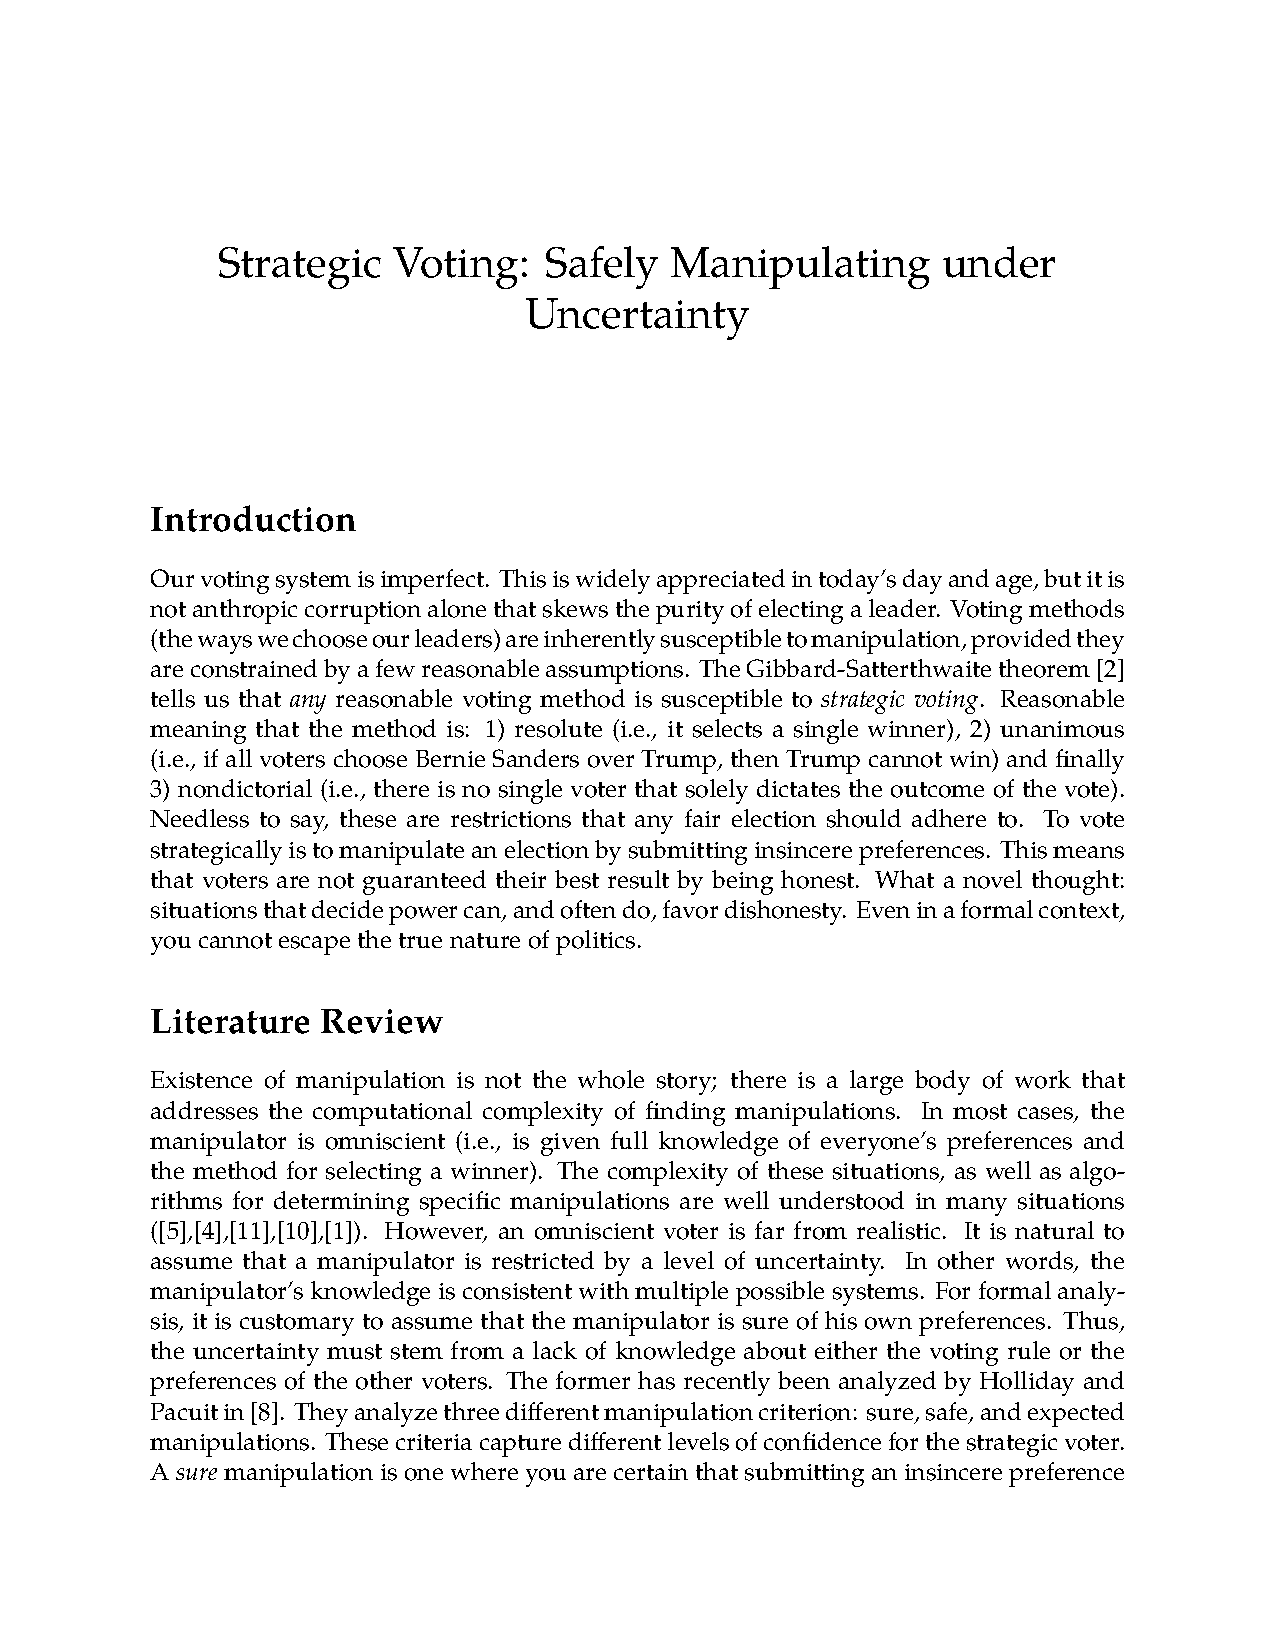
\includepdf[pages=-]{SV.pdf}
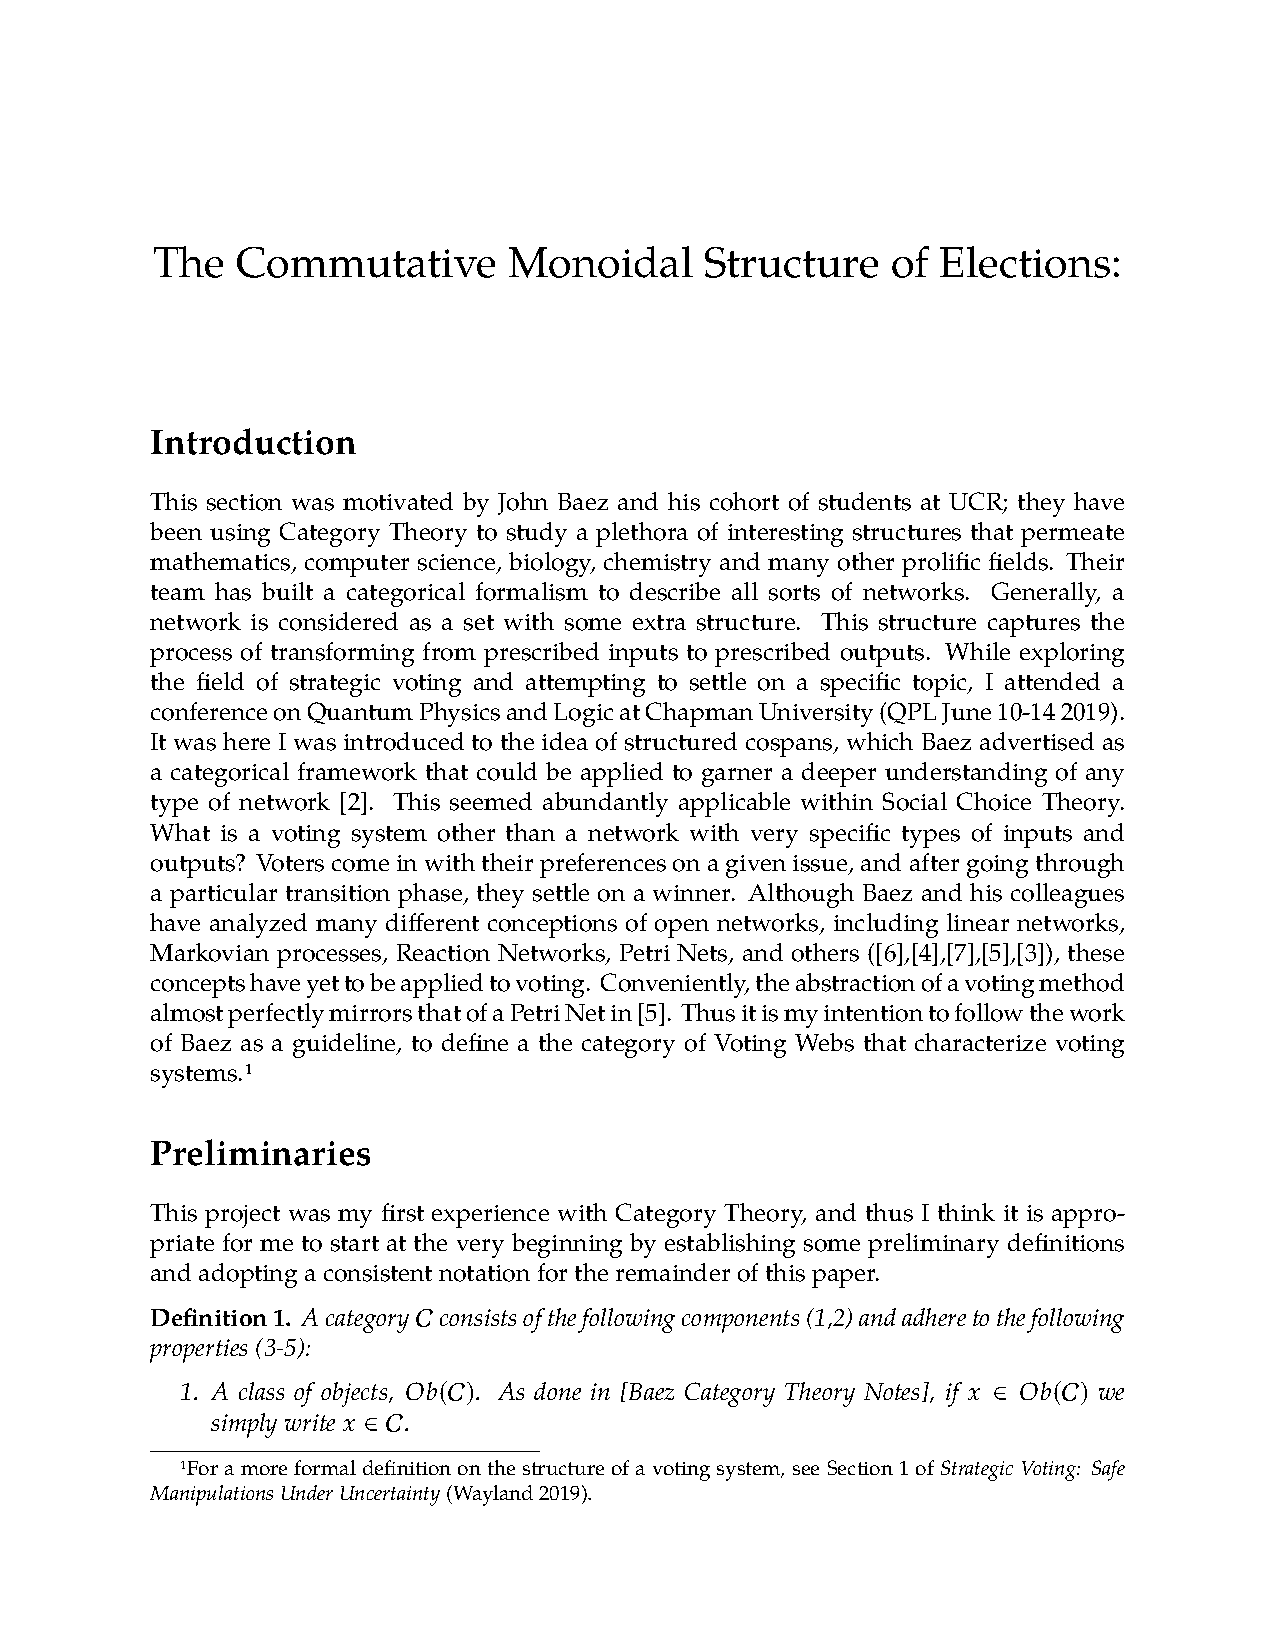
\includepdf[pages=-]{vw.pdf}


\end{document}